\documentclass[a4paper, 11pt]{article}
\usepackage{comment} % enables the use of multi-line comments (\ifx \fi)
\usepackage{fullpage} % changes the margin
\usepackage{url}
\usepackage{graphicx}
\usepackage{caption}
\usepackage{booktabs}
\usepackage{amsmath}

\DeclareMathOperator*{\argmin}{argmin} 

\begin{document}
\noindent
\large\textbf{Deep Learning Course 2017} \hfill \textbf{Ilia Dobrusin} \\
 Autonomous Intelligent Systems \hfill \textbf{Archit Basal} \\
 University Freiburg \hfill Due Date: 22.01.2017

\section*{Deep Learning Lab Course 2017 - Exercise 4}
This assignment consists of two parts: manually simulating Q-learning and implementing Deep Q-learning using Tensorflow. 

\section{Manual Q-Learning}
\subsection*{Q-function update rule}
 Update rule for the Q function for any state-action pair:
 \begin{equation*}
    Q(i, u) = (1 - \gamma) * Q(i, u) + \gamma * (r(i, u) + \argmin_{u'} Q(j, u'))    
  \end{equation*}
where $i$ is the initial state, $u$ is the action taken in $i$, $j$ the final state reached from $i$ by action $u$, and $r$ is the reward function.


The goal state can be made an absorbing state by ensuring that all actions leading away from the goal state return the agent to the goal state, i.e. for all $u$ available in $g$, where $g$ is the goal state, the transition function $T$ is defined as $T(g, u) = g$. Another way to deal with this is to introduce an action to \textit{stay} in the current state, and ensure that all actions except the \textit{stay} action have a large penalty whereas the \textit{stay} action has a reward of $0$. Although it must be noted that the \textit{stay} action can be considered a \textit{noop} that can lead to other complications unless properly handled, for example, the \textit{stay} action should result in a small penalty in all non-goal states, and not be $0$.

\subsection*{Moving in maze}
Assuming that the cell the agent starts in is represented by $(0,0)$, such that the goal state is the cell $(2,0)$, the wall is the cell $(1,0)$ and the cell immediately below $(0,0)$ is $(0,1)$, the following sequence of state-action pairs would be updated:
\begin{equation*}
<(0,0), D>, <(0,1), R>, <(1,1), U>, <(1,1), R>, <(2,1), U>
\end{equation*}
where the actions available to the agent are to move up, down, left or right, represented with U, D, L and R respectively.

Since the learning rate is 1, the old values of the Q-function will be completely ignore during the update step and only the sum of the reward and the Q-value of the next state and it's greedily-selected best action will be retained. Assuming the Q-function was initialized with zeroes, the updated Q-values will be: 
\begin{center}
  $Q((0,0), D) = -1$ \\
  $Q((0,1), R) = -1$ \\ 
  $Q((1,1), U) = -1$ \\   
  $Q((1,1), R) = -1$ \\  
  $Q((1,2), U) = -1$ \\
\end{center}

and Q(i, u) = 0 for all other valid combinations of i and u.

\section{Deep Q-learning}
The second part of the assignment consists of implementing Deep Q-learning using a neural network for predicting the Q-value for a given state. The network is similar to the approach of the visual planner from assignment 3, although the architecture is simplified, with fewer layers and no max-pooling layers. Figure \ref{fig:nn_arch} shows the architecture of the network.

\subsection*{Setup and Hyperparameters}
The agent moved in the environment at random for 1000 steps in order to build a up a transition table prior to training. In addition, the agent performs random movements with a certain probability, which decayed after each training step, resulting in less random movements of the agent as the training progresses. The network was trained with the hyperparameters shown in table \ref{tbl:hyperparameters}.

\begin{table}[ht]
	\centering
    \footnotesize
	\begin{tabular}{cl}
		\toprule
		\textbf{Parameter}	&	\textbf{Value} \\
		\midrule
        Discount factor 	&	0.99 \\
        Max. exploration probability & 0.7 \\
        Min. exploration probability & 0.2 \\
        Exploration probability decay  & 0.99999 \\
        \midrule
        & (steps)\\
        Exploration steps prior to training 	&	1,000 \\
        Total training steps 	&	20,000 \\
		\bottomrule
    \end{tabular}
    \caption{Hyperparameters used during training}
    \label{tbl:hyperparameters}
\end{table}

\subsection{Issues during implementation}
At first, we implemented DQN using Keras, which resulted in suboptimally trained model where the agent would reach state next to goal state without moving to the goal state. In the end, we implemented the network using Tensorflow, which lead to an agent who could reach the goal. The training process in itself is instable in the sence that small changes in the architecture lead to significantly worse results, were the calculated Q-loss explodes to values up to a range of $10^{20}$, while for a successful run the loss is in the range between 0 and 20.  \\
Our first approach consisted of a target network as described by Wang et al \cite{Wang15}, but due to changing from Keras to Tensorflow we did not reimplement it the final architecture.\\
In the current state, the architecture is not yielding good results on every run.

\subsection*{Results}
The network was trained using hyperparameters in table \ref{tbl:hyperparameters}. 
Figure \ref{fig:acc_rew_train} shows the accumulated reward during training. As the accumulated reward does not increase over time, it is possible that the model did not yet converge. We would expect the curve to rise after the model is trained sufficiently, although overfitting could occur. In figure \ref{fig:train_loss} the loss during training of the first 1000 episodes after the exploration phase is displayed. Figure \ref{fig:acc_rew_test} shows the resulting accumulated rewards during testing, where the agent performed 10000 steps, reaching the goal in 96,71\% episodes.


\begin{figure}[ht!]
    \centering
    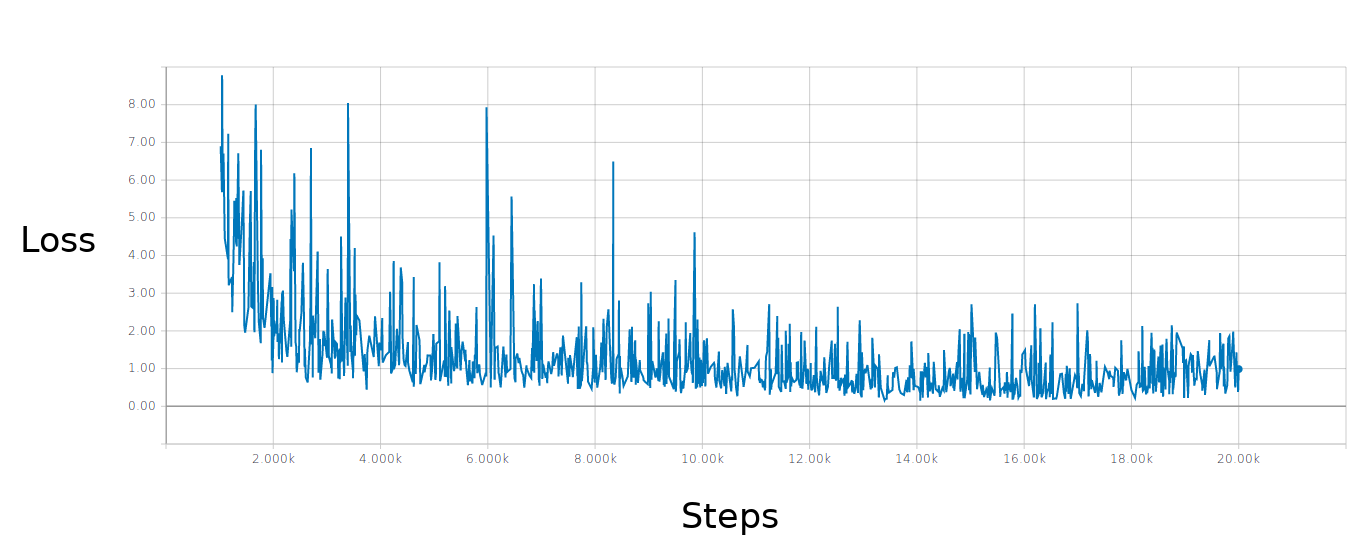
\includegraphics[width=16cm]{images/loss.png}
        \caption{Loss after each training step over the training time.}
        \label{fig:train_loss}
\end{figure}

\begin{figure}[ht!]
    \centering
    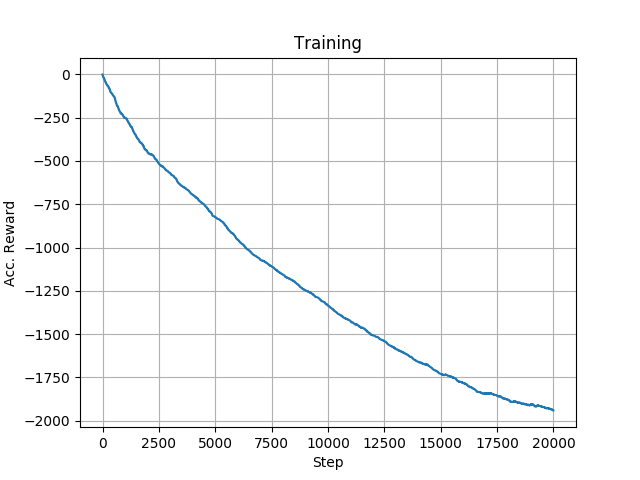
\includegraphics[height=8cm]{images/acc_reward_train.png}
        \caption{Accumulated reward during training}
        \label{fig:acc_rew_train}
\end{figure}

\begin{figure}[ht!]
    \centering
    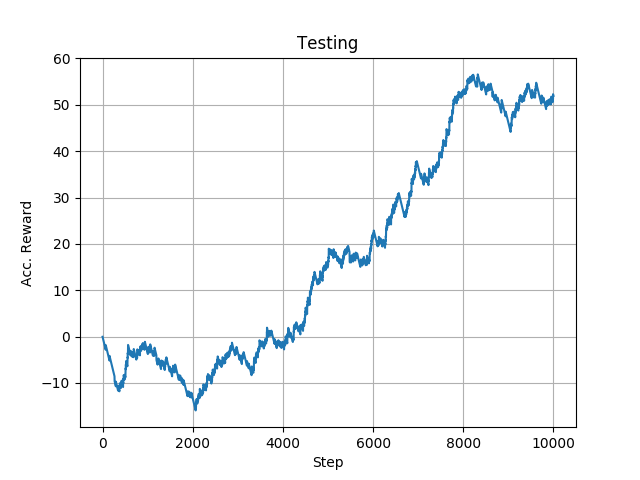
\includegraphics[height=8cm]{images/acc_reward_test.png}
        \caption{Accumulated reward during testing}
        \label{fig:acc_rew_test}
\end{figure}

\begin{figure}[ht!]
    \centering
    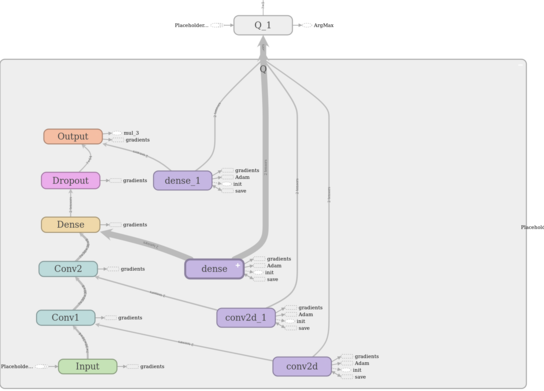
\includegraphics[height=8cm]{images/arch.png}
        \caption{The architecture of the neural network used in this exercise}
        \label{fig:nn_arch}
\end{figure}
\clearpage
\bibliographystyle{abbrv}
\bibliography{bib.bib}

\end{document}
